\chapter{Ovládání}
\label{7-aplikace}
Pro ovládání drona byla vytvořena jednoduchá aplikace pro Adroid. Aplikace byla napsána v programovacím jazyku Java a programovacím prostředí Android studio.\\

Aplikace využívá Bluetooth, GNSS mobilu. Přes bluetooth modul probíhá přenos dat pro ovládání drona, GNSS slouží pro zjištování polohy uživatele a zobrazeí na widgetu Google Maps.\\

\section{Hlavní obrazovka}
Při otevření aplikace se na display zobrazí hlavní obrazovka. Zde má uživatel na výběr zda využije manuální či autonomní ovládání. Po rozklikknutí jednoho ze spárovaných bluetooth zařízení, aplikace otevře okno pro ovládání.\\
\begin{figure}[h]
	\centering
	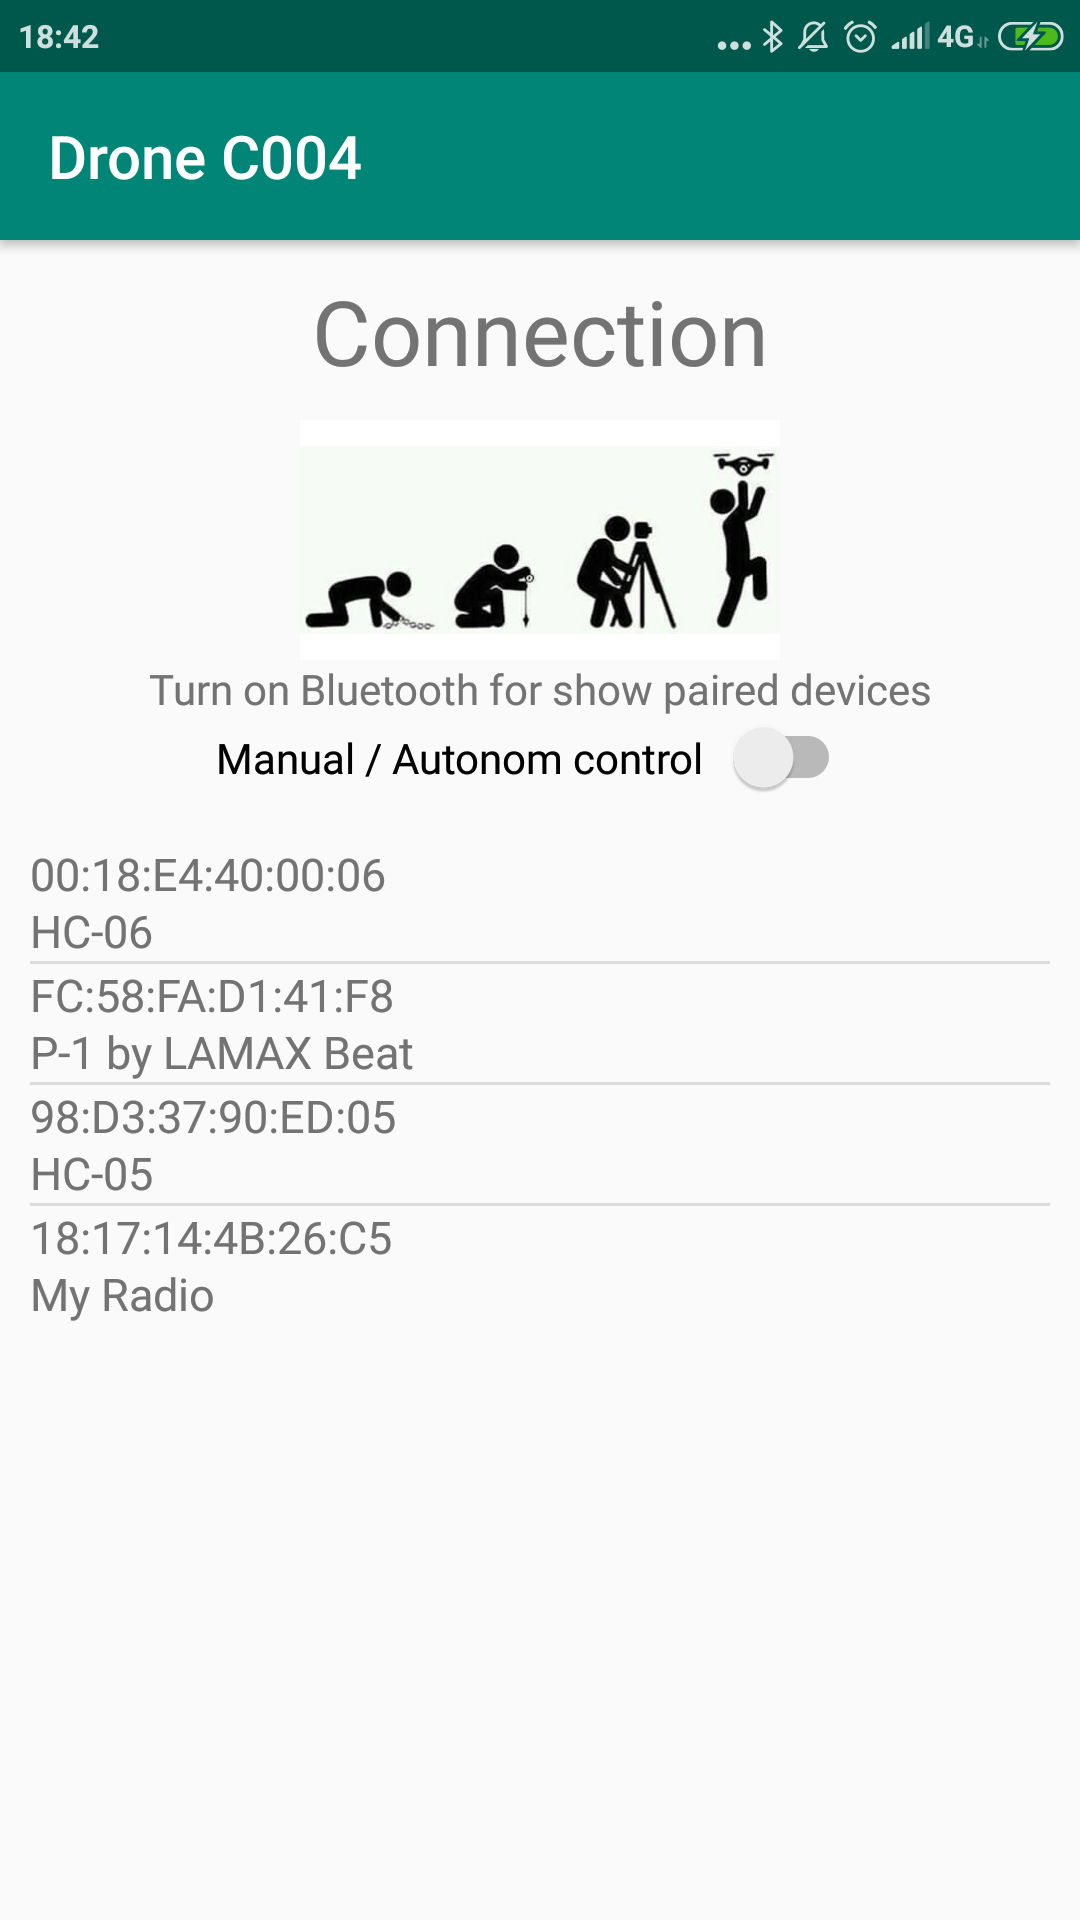
\includegraphics[width=6cm]{pictures/app1.png}
	\caption{Screenshoot hlavní obrazovky}
\end{figure}

\section{Manuální ovládání} 
Manuální ovladání funguje totožně jako RC soustava. Levý joystick slouží k ovládání náklonů pitch a roll, pravý joystick složí k ovládání throttle a yaw. 

\begin{figure}[h]
	\centering
	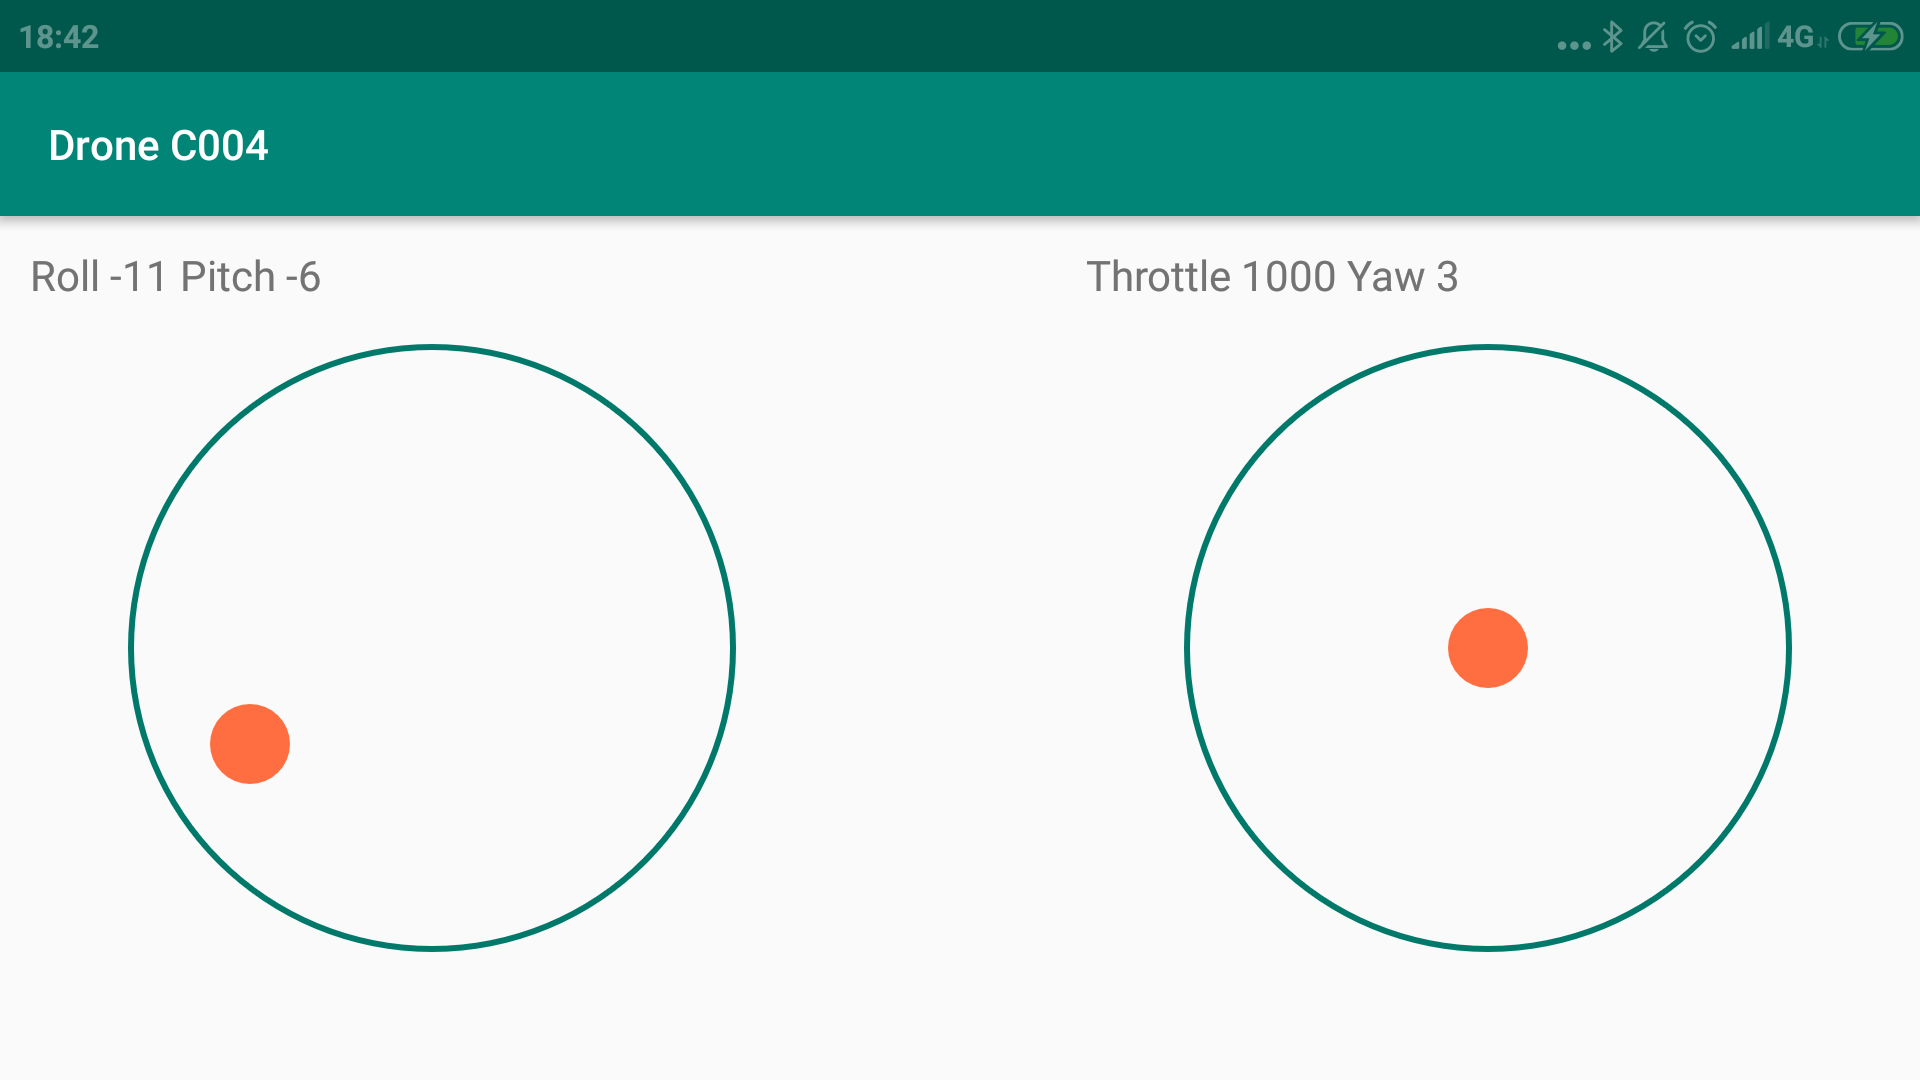
\includegraphics[width=10cm]{pictures/app.png}
	\caption{Schreenshoot obrazovky pro manuální ovládání}
\end{figure}

\begin{figure}[h]
	\centering
	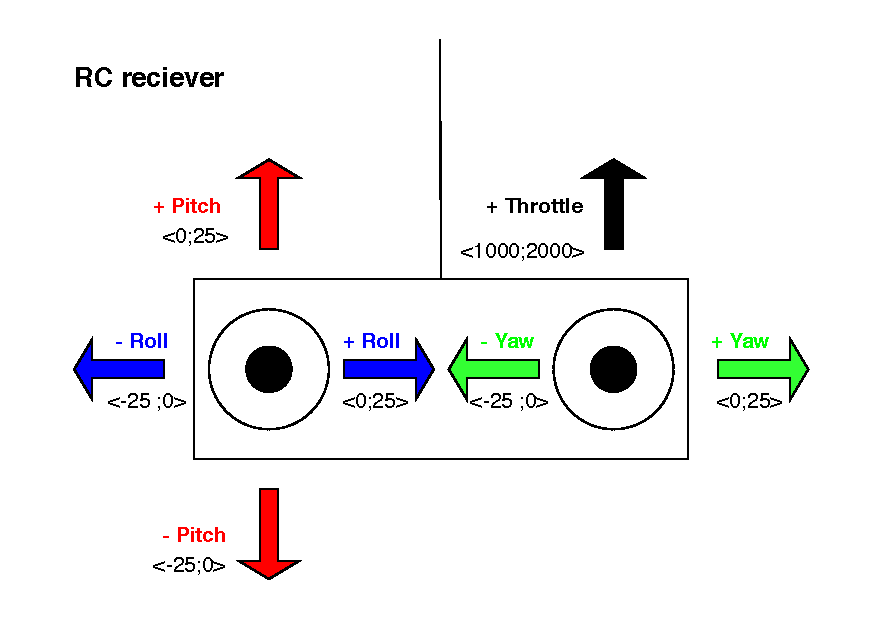
\includegraphics[width=14cm]{pictures/rcDiagram.pdf}
	\caption{Diagram RC soustavy}
\end{figure}

\section{Autonomní ovládání} 
Pro autonomní ovládání stačí pouze zadat souřadnice v systému WGS-84. Přes tlačítko SEND je zaslat dronovi a uživatel může na mapě sledovat, kde se dron nachází. Spodní tlačítko Home slouží k návratu drona a startovní místo.

\begin{figure}[h]
	\centering
	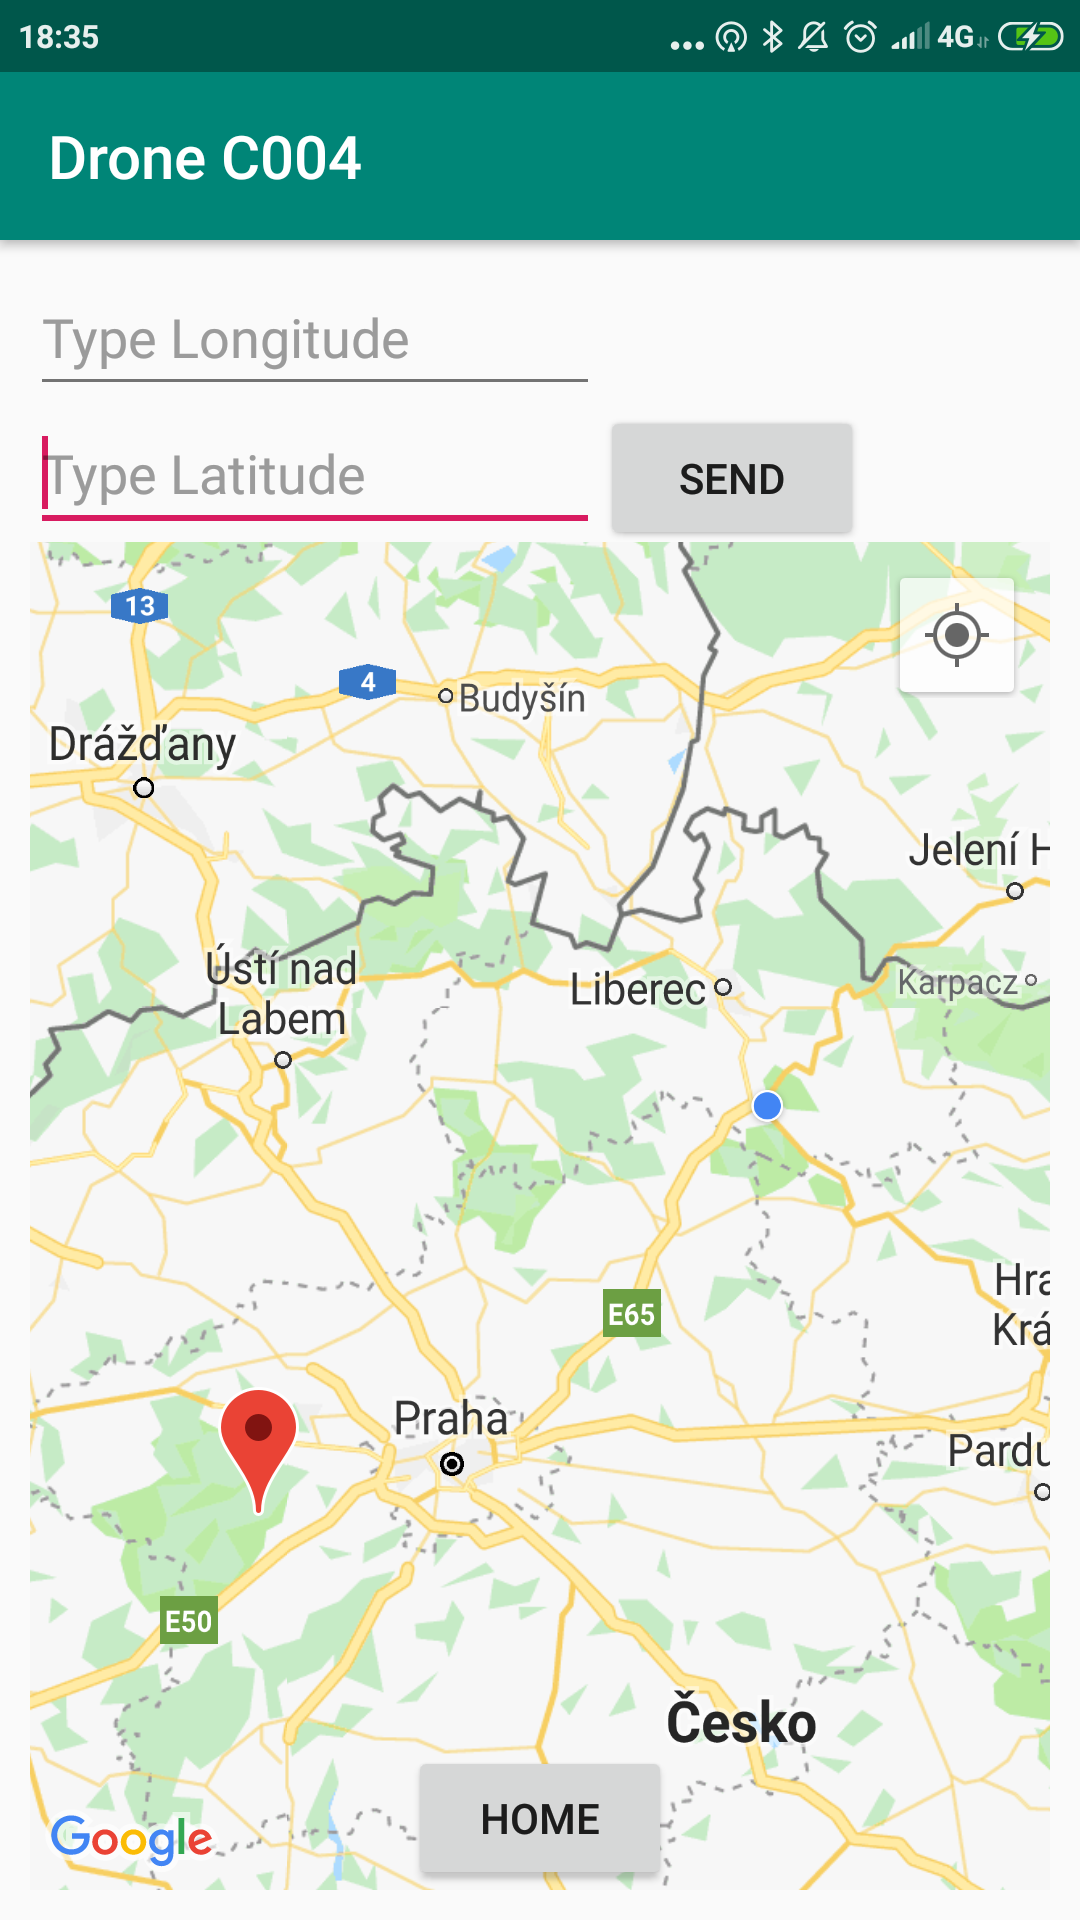
\includegraphics[width=6cm]{pictures/app2.png}
	\caption{Schreenshoot obrazovky pro autonomní ovládání}
\end{figure}

